\PassOptionsToPackage{usenames,dvipsnames,table,x11names}{xcolor}
\documentclass[8pt]{beamer}

% SETTING THEMES ----------------------------------------
%\usetheme{Warsaw}
\usetheme{Luebeck}
%\usetheme{Boadilla}

% COLORS IN PRESENTATION --------------------------------
\setbeamercolor*{palette primary}{bg = Firebrick1, fg = white}


%https://www.tug.org/pracjourn/2007-4/walden/color.pdf
%https://tex.stackexchange.com/questions/368784/change-color-in-beamer-theme

% FONT --------------------------------------------------
%\usefonttheme{professionalfonts} %doesn't do anything?
\usefonttheme{serif}

% CHANGING ITEMIZE ITEMS --------------------------------
\setbeamertemplate{itemize item}{\color{black} $\vcenter{\hbox{\tiny$\bullet$}}$} %style of item
\setbeamertemplate{itemize subitem}{\tiny \color{black}$\blacktriangleright$} %style for sub item
\setbeamercolor{itemize item}{fg=black} %changes color of all items

\setbeamertemplate{enumerate items}[default] %default number style
\setbeamercolor{enumerate item}{fg=black}

%\setbeamerfont{frametitle}{size=\Large}

%https://tex.stackexchange.com/questions/59742/progress-bar-for-latex-beamer

%\insertframenumber/\inserttotalframenumber

%getting rid of stuff on bottom
\setbeamertemplate{footline}[frame number]{}
\setbeamertemplate{navigation symbols}{}
%\setbeamertemplate{footline}{%
%    \raisebox{5pt}{\makebox[\paperwidth]{\hfill\makebox[20pt]{\color{gray}
%          \scriptsize\insertframenumber/\inserttotalframenumber}}}\hspace*{5pt}}

%\usepackage{natbib}
%\renewcommand\bibfont{\scriptsize}
\setbeamercolor*{bibliography entry title}{fg=black}
\setbeamercolor*{bibliography entry author}{fg=black}
\setbeamercolor*{bibliography entry location}{fg=black}

%\newcommand*{\myfont}{\fontfamily{phv}\selectfont} %helvecta
\newcommand*{\myfont}{\fontfamily{crm}\selectfont} %cm wont change
%https://tex.stackexchange.com/questions/25249/how-do-i-use-a-particular-font-for-a-small-section-of-text-in-my-document

%%%%%%%%%%%%%%%%%%%%%%%%%%%%%%%%%%%%%%%%%%%%%%%%%%%%%%%%%%
%%%%%%%%%%%%%%%%%%%%%%%%%%%%%%%%%%%%%%%%%%%%%%%%%%%%%%%%%%
%%%%%%%%%%%%%%%%%%%%%%%%%%%%%%%%%%%%%%%%%%%%%%%%%%%%%%%%%%

%------------------------------------------------------
%                Math Packages
%------------------------------------------------------

%\usepackage[intlimits]{amsmath}
\usepackage{amsmath}
\usepackage{amssymb}
\usepackage{amsthm}
%\everymath{\displaystyle}
\usepackage{siunitx} % for SI units (e.g. C, degree)
\usepackage{bm} % bold for some math symbols
\usepackage{nicefrac} % for nicer fractions sometimes
\usepackage[thinc]{esdiff} % for derivatives

%------------------------------------------------------
%                Tikz and Pgfplots
%------------------------------------------------------

\usepackage{pgfplots}
\usepackage{tkz-euclide}
\pgfplotsset{compat=1.15}
\usetikzlibrary{arrows,shadows,positioning, calc, decorations.markings, hobby, quotes,angles,decorations.pathreplacing,intersections, matrix,backgrounds}
\usepgfplotslibrary{polar,colormaps,fillbetween}
\usepgflibrary{shapes.geometric}
%\usetkzobj{all}

%------------------------------------------------------
%                Formatting
%------------------------------------------------------

% COLORS ----------------------------------------------
%\usepackage[dvipsnames, table]{xcolor}
\usepackage{xcolor}

% FIGURES ---------------------------------------------
\usepackage{graphicx} % for importing images
\usepackage{subcaption} % for making subfigures
\usepackage[labelfont=bf]{caption} % changing style of figures
% use font=it for italic font

% PAGE LAYOUT -----------------------------------------
%\linespread{1.3} % changes line spacing
\setlength{\parskip}{0.75em}

%\usepackage{indentfirst}
%\usepackage{parskip} % for not indenting paragraphs first
\usepackage{multirow} % having multiple rows
\usepackage{multicol} % having multiple columns
\usepackage[T1]{fontenc} % can combine \sc and \bf font

% LANGUAGES -------------------------------------------
\usepackage[english]{babel} % for correctly using english
\usepackage[utf8x]{inputenc} % compiling correctly
\usepackage{CJK} % using Chinese, Japanese, and Korean

% MISC ------------------------------------------------
\usepackage[normalem]{ulem} % for \sout
\usepackage{tikzsymbols} % for emojis
\usepackage{booktabs,eqparbox} % for tables
\usepackage{verbatim} % for verbatim environment

%------------------------------------------------------
%                Custom Commands
%------------------------------------------------------

\newcommand{\done}{\hfill $\square$ \vspace{1cm}}
\newcommand{\csch}{\mathrm{csch}}
\newcommand{\sech}{\mathrm{sech}}

%\newcommand{\dd}{\mathop{}\,\mathrm{d}}
\newcommand{\dd}{\;\mathrm{d}}

% COLOR CODING -----------------------------------------------
\newcommand{\code}[1]{\textcolor{Bittersweet}{\texttt{#1}}} % using for emphasizing variables, code, etc.
\newcommand{\mydef}[1]{\textcolor{SteelBlue3}{\textit{#1}}} % defining something

% VENN DIAGRAMS ----------------------------------------------
\def\firstcircle{(90:1.75cm) circle (2.5cm)}
\def\secondcircle{(210:1.75cm) circle (2.5cm)}
\def\thirdcircle{(330:1.75cm) circle (2.5cm)}
\def\sampspace{(-6,-4.25) rectangle (6,5)}  %Cartesian
%\def\sampspace{(225:7cm) rectangle (45:7cm)} %polar

% TO DO LIST -------------------------------------------------
%\usepackage{enumitem}

%\newlist{todolist}{itemize}{2}
%\setlist[todolist]{label=$\square$}

%\usepackage{pifont}
%\newcommand{\cmark}{\ding{51}}%
%\newcommand{\xmark}{\ding{55}}%
%\newcommand{\fin}{\rlap{$\square$}{\raisebox{2pt}{\color{Green}{\large\hspace{1pt}\cmark}}}%
%\hspace{-2.5pt}}
%\newcommand{\wontfix}{\rlap{$\square$}{\color{red}{\large\hspace{1pt}\xmark}}}

%------------------------------------------------------
%                Custom Environments
%------------------------------------------------------

\usepackage{mdframed}

% EXERCISE -------------------------------------------------
\mdfdefinestyle{exercise}{
	backgroundcolor=black!10,roundcorner=8pt,hidealllines=true,nobreak
}

%\begin{mdframed}[style=exercise]
%\end{mdframed}

% MATHEMATICA ------------------------------------------------
\mdfdefinestyle{mathematica}{
	backgroundcolor=Tan!15,roundcorner=8pt,hidealllines=true,nobreak,fontcolor=Bittersweet
}

% R ---------------------------------------------------------
\mdfdefinestyle{R}{
	backgroundcolor=SteelBlue3!15, roundcorner=8pt, hidealllines=true, nobreak, fontcolor=SteelBlue3
}

% R ---------------------------------------------------------
\mdfdefinestyle{python}{
	backgroundcolor=Green!15, roundcorner=8pt, hidealllines=true, nobreak, fontcolor=Green
}


\definecolor{Auburn}{rgb}{0.25, 0.1, 0}

%\usepackage[style=authoryear]{biblatex}

%%%%%%%%%%%%%%%%%%%%%%%%%%%%%%%%%%%%%%%%%%%%%%%%%%%%%%%%%%
%%%%%%%%%%%%%%%%%%%%%%%%%%%%%%%%%%%%%%%%%%%%%%%%%%%%%%%%%%
%%%%%%%%%%%%%%%%%%%%%%%%%%%%%%%%%%%%%%%%%%%%%%%%%%%%%%%%%%





\title{REU 2019 Presentation}
\author{Regularization Techniques Applied to Genomic Data}
\institute{
\includegraphics[]{lamar_logo.jpeg}}
\date{Aiden Kenny, Danielle Solomon\\[0.5pt]
Lamar University\\[0.5pt]
\today}
    
\begin{document}

%%%%%%%%%%%%%%%%%%%%%%%%%%%%%%%%%%%%%%%%%%%%%%%%%%%%%%%%%%
%%%%%%%%%%% TITLE FRAME %%%%%%%%%%%
%%%%%%%%%%%%%%%%%%%%%%%%%%%%%%%%%%%%%%%%%%%%%%%%%%%%%%%%%%

\begin{frame}

\maketitle

\end{frame}

%%%%%%%%%%%%%%%%%%%%%%%%%%%%%%%%%%%%%%%%%%%%%%%%%%%%%%%%%%
%%%%%%%%%%% FRAME 1 %%%%%%%%%%%
%%%%%%%%%%%%%%%%%%%%%%%%%%%%%%%%%%%%%%%%%%%%%%%%%%%%%%%%%%

\begin{frame}{Introduction}

\mydef{Statistical learning} refers to various techniques used to understand data. %\pause

When data is collected, we store it in a \mydef{data matrix} $\mathbf{X}_{n \times p}$. %\pause
\begin{itemize}
    \item Each row $\bm{x}_i$ of the matrix are the values for each observation. %\pause
    \item Each column $\mathbf{x}_j$ of the matrix are the values of a predictor for all observations. %\pause
\end{itemize}

There is usually some response that is measured with each observation, and we store them in the \mydef{response vector} $\mathbf{y}$. %\pause

Our goal is to fit a \mydef{statistical model} $f(\bm{x})$ that can use $\mathbf{X}$ to \mydef{predict} $\mathbf{y}$! %\pause
\begin{itemize}
    \item We store these predictions in a \mydef{prediction vector} $\hat{\mathbf{y}} = (f(\bm{x}_1), \ldots, f(\bm{x}_n))$. %\pause
    \item This is known as \mydef{supervised learning}, where we have a response that can be measured. %\pause
\end{itemize}

There are two goals for a statistical model: %\pause
\begin{enumerate}
    \item \mydef{Prediction}: we want our predictions $\hat{\mathbf{y}}$ to be accurate.
    \item \mydef{Interpretation}: we want to know which predictors are important in determining the response.
\end{enumerate}

    
\end{frame}



\begin{frame}{$\ldots$}
In a general sense, we have two types of statistical models: %\pause
\begin{enumerate}
    \item \mydef{Regression models}: the response is continuous (we will focus on this one). %\pause
    \item \mydef{Classification models}: the response is categorical. %\pause
\end{enumerate}

How do we know our model predicts accurately? %\pause
\begin{itemize}
    \item For regression, we can use the \mydef{mean-squared error}, $\displaystyle \mathrm{MSE} = \frac{1}{n} \| \mathbf{y} - \hat{\mathbf{y}} \|_2^2$. %\pause
    \item For classification, we can use the \mydef{error rate}, $\displaystyle \mathrm{ER} = \frac{1}{n} \sum_{i=1}^{n} \mathbb{I}(y_i \not= \hat{y}_i)$. %\pause
    \item We want these to be as low as possible! %\pause
\end{itemize}

We want to avoid our models from \mydef{over-fitting}, so we do this: %\pause
\begin{enumerate}
    \item Randomly divide the data into a training set $\mathbf{X}_{\mathcal{R}}$ and a test set $\mathbf{X}_{\mathcal{T}}$. %\pause
    \item We fit $f(\bm{x})$ using the test set $\mathbf{X}_{\mathcal{R}}$. %\pause
    \item We check the prediction accuracy using the training set $\mathbf{X}_{\mathcal{T}}$. The best models will have the lowest \mydef{test error}. %\pause
\end{enumerate}
    
\end{frame}

\begin{frame}{Flexibility and the Bias-Variance Trade-Off}

Loosely speaking, a statistical learning method is \mydef{flexible} if it is able to fit a wide variety of forms for $f(\bm{x})$. %\pause
\begin{itemize}
    \item The more flexible a model becomes, the more parameters that need to be estimated! %\pause
    \item The more flexible a model is, the less interpretable! %\pause
    \item If model is too flexible, it will also over-fit! %\pause
\end{itemize}

There are two main characteristics of a statistical model: %\pause
\begin{enumerate}
    \item \mydef{Bias}: the error introduced by estimating a more complicated model with a simpler model. %\pause
    \item \mydef{Variance}: how much the model would change if it were fit using a different training set. %\pause
\end{enumerate}

As a model becomes more flexible, its bias will \textit{decrease} while its variance will \textit{increase}! %\pause

There is a flexibility ``sweet-spot'' where both the bias and variance are low enough to have the lowest test error; this is known as the \mydef{bias-variance trade-off}.
    
\end{frame}

\begin{frame}{$\ldots$}

\begin{columns}

\column{0.6\textwidth}
\begin{figure}
    \centering
    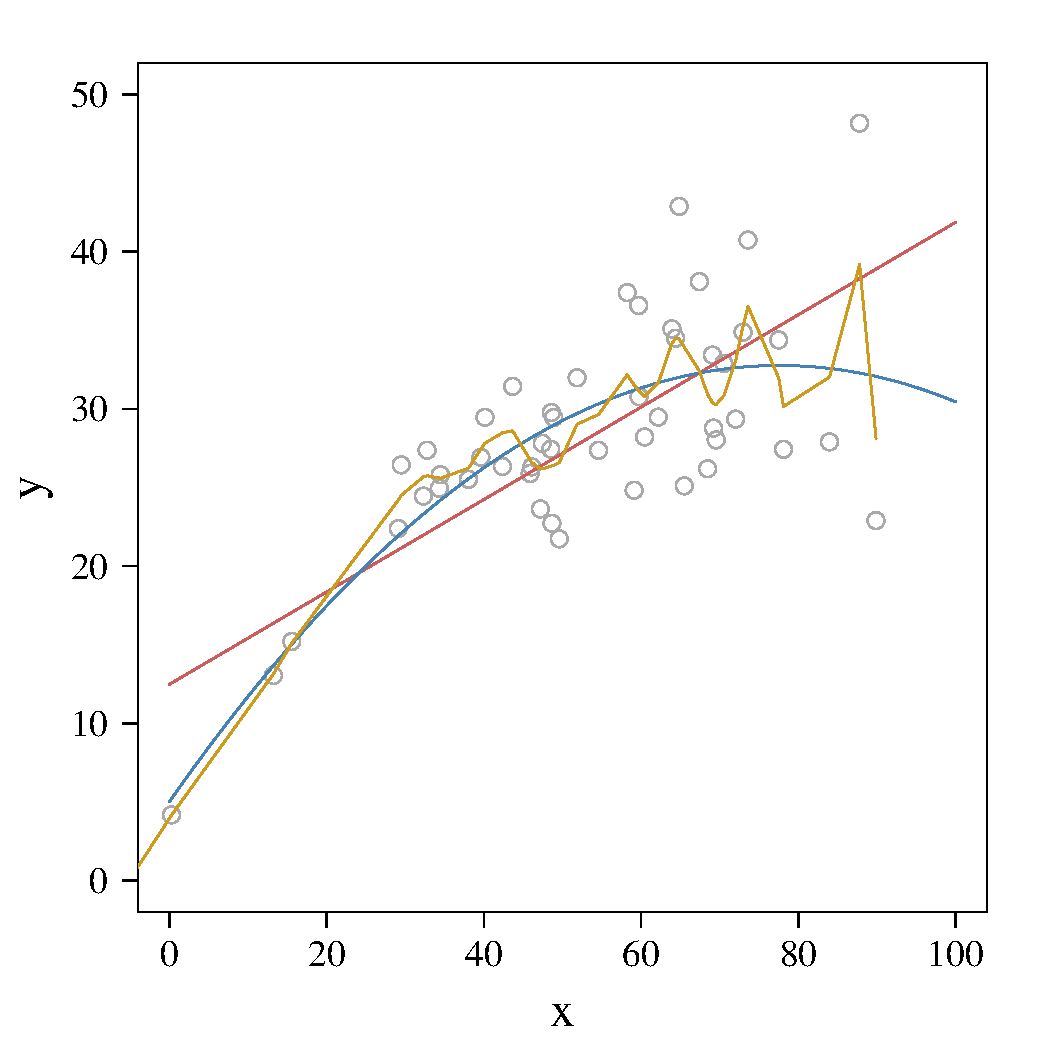
\includegraphics[width=1\textwidth]{model_flex.pdf}
    %\caption{Caption}
    \label{model_flex}
\end{figure} %\pause

\column{0.39\textwidth}
\begin{itemize}
    \item The \textcolor{IndianRed3}{red} line has \textit{low} flexibility: high bias and low variance. 
    \item The \textcolor{SteelBlue4}{blue} line has \textit{medium} flexibility: medium bias and variance. 
    \item The \textcolor{Goldenrod3}{orange} line has \textit{high} flexibility: low bias and high variance. 
\end{itemize}

\end{columns}
    
\end{frame}

\begin{frame}{Ordinary Least-Squares and its Problems}

The \mydef{linear regression} model has the form 
\begin{align*}
    f(\bm{x}) = \beta_0 + \bm{x}^T \bm{\beta},
\end{align*}
where $\beta_0$ and $\bm{\beta} = (\beta_1,\ldots,\beta_p)$ are the \mydef{parameters} that must be estimated from the data. %\pause

The coefficients can be solved by minimizing the \mydef{residual sum-of-squares}
\begin{align*}
    \mathrm{RSS}(\beta_0, \bm{\beta}) = \| \mathbf{y} - \beta_0 \mathbf{1} - \mathbf{X} \bm{\beta} \|_2^2.
\end{align*}

There are some problems with this approach: %\pause
\begin{itemize}
    \item As $p$ increases, the model becomes extremely variable, and when $n < p$, there is no unique solution to $\hat{\bm{\beta}}$! %\pause
    \item When $p$ becomes large, the model becomes less interpretable. %\pause
\end{itemize}

We will use \mydef{regularization} to help us out!

    
\end{frame}

\begin{frame}{Regularization}

Regularization (a.k.a. \mydef{shrinkage}) involves shrinking the estimated coefficients $\hat{\bm{\beta}}$ toward zero. %\pause
\begin{itemize}
    \item The goal is to have a \textit{small} increase in bias to give a \textit{large} decrease in variance! %\pause
    \item There are various shrinkage estimation techniques. %\pause
\end{itemize}

There are some things that are standard to all regularization techniques: %\pause
\begin{itemize}
    \item We always \mydef{center} the data, such that the average value for each predictor $\mathbf{x}_j$ is zero. %\pause
    \item As a result, the intercept coefficient is estimated by $\displaystyle \hat{\beta}_0 = \frac{1}{n} \sum_{i=1}^n y_i$. So we are only shrinking $\bm{\beta} = (\beta_1,\ldots,\beta_p)$. %\pause
\end{itemize}

These can be applied to a wide variety of models, but this presentation will focus on linear regression!
    
\end{frame}

\begin{frame}{Ridge Regression}

\mydef{Ridge Regression} \cite{hoerl1970ridge} shrinks the coefficients by imposing a \textit{squared} $\ell_2$ norm on $\bm{\beta}$. The estimates are found by minimizing the loss function 
\begin{align*}
    J(\bm{\beta}) = \frac{1}{2} \| \mathbf{y}  - \mathbf{X} \bm{\beta} \|_2^2 + \lambda \| \bm{\beta} \|_2^2.
\end{align*} %\pause
$\lambda$ is a \mydef{tuning parameter} which affects the severity of the shrinkage (larger values correspond to more shrinkage). %\pause

Can also be viewed as minimizing the loss function 
\begin{align*}
    J(\bm{\beta}) = \frac{1}{2} \| \mathbf{y}  - \mathbf{X} \bm{\beta} \|_2^2 ~~\text{ subject to }~~ \| \bm{\beta} \|_2^2 \le t,
\end{align*}
for some constant $t$. %\pause
\begin{itemize}
    \item This constraint is known as the \mydef{shrinkage penalty}.
\end{itemize}

The main drawback to ridge regression is that \textit{the estimated coefficients will almost never equal 0}. %\pause
\begin{itemize}
    \item In other words, ridge regression results in \mydef{dense} models, since none of the predictors are left out. %\pause
    \item May be okay for prediction, but bad for interpretability!
\end{itemize}
    
\end{frame}


\begin{frame}{The Lasso}

The \mydef{lasso} \cite{tibshirani1996regression} shrinks the coefficients by imposing an $\ell_1$ norm on $\bm{\beta}$. The estimates are found by minimizing the loss function
\begin{align*}
    J(\bm{\beta}) = \frac{1}{2} \| \mathbf{y}  - \mathbf{X} \bm{\beta} \|_2^2 + \lambda \| \bm{\beta} \|_1.
\end{align*} %\pause
Can also be viewed as minimizing the loss function 
\begin{align*}
    J(\bm{\beta}) = \frac{1}{2} \| \mathbf{y}  - \mathbf{X} \bm{\beta} \|_2^2 ~~\text{ subject to }~~ \| \bm{\beta} \|_1 \le t,
\end{align*}
for some constant $t$. %\pause

The main selling point of the lasso is that \textit{many of the irrelevant coefficients will forcibly be set to zero}. %\pause
\begin{itemize}
    \item In other words, the lasso provides \mydef{feature selection} by selecting the most important predictors. %\pause
    \item Great for interpretability, especially when $p$ is large!
\end{itemize}

    
\end{frame}

\begin{frame}{The Elastic Net}

The \mydef{elastic net} \cite{zou2005regularization} is a generalization of the lasso and ridge regression. The estimates are found my minimizing the loss function 
\begin{align*}
    J(\bm{\beta}) = \frac{1}{2} \| \mathbf{y}  - \mathbf{X} \bm{\beta} \|_2^2 + \lambda \Big[ \alpha \| \bm{\beta} \|_1 + (1 - \alpha) \| \bm{\beta} \|_2^2 \Big],
\end{align*}
for $0 \le \alpha \le 1$. %\pause

Can also be viewed as minimizing the loss function 
\begin{align*}
    J(\bm{\beta}) = \frac{1}{2} \| \mathbf{y}  - \mathbf{X} \bm{\beta} \|_2^2 ~~\text{ subject to }~~ \alpha \| \bm{\beta} \|_1 + (1 - \alpha) \| \bm{\beta} \|_2^2\le t,
\end{align*}
for some constant $t$. %\pause
\begin{itemize}
    \item $\alpha = 0$ corresponds to ridge regression, while $\alpha = 1$ corresponds to the lasso. %\pause
\end{itemize}

Why would we want such a compromise? %\pause
\begin{itemize}
    \item Best of both worlds -- performs feature selection like the lasso, and shrinks correlated coefficients like ridge regression! %\pause
    \item Also has computational shortcuts. 
\end{itemize}
    
\end{frame}

\begin{frame}{Contour Plots}

\begin{figure}
    \centering
    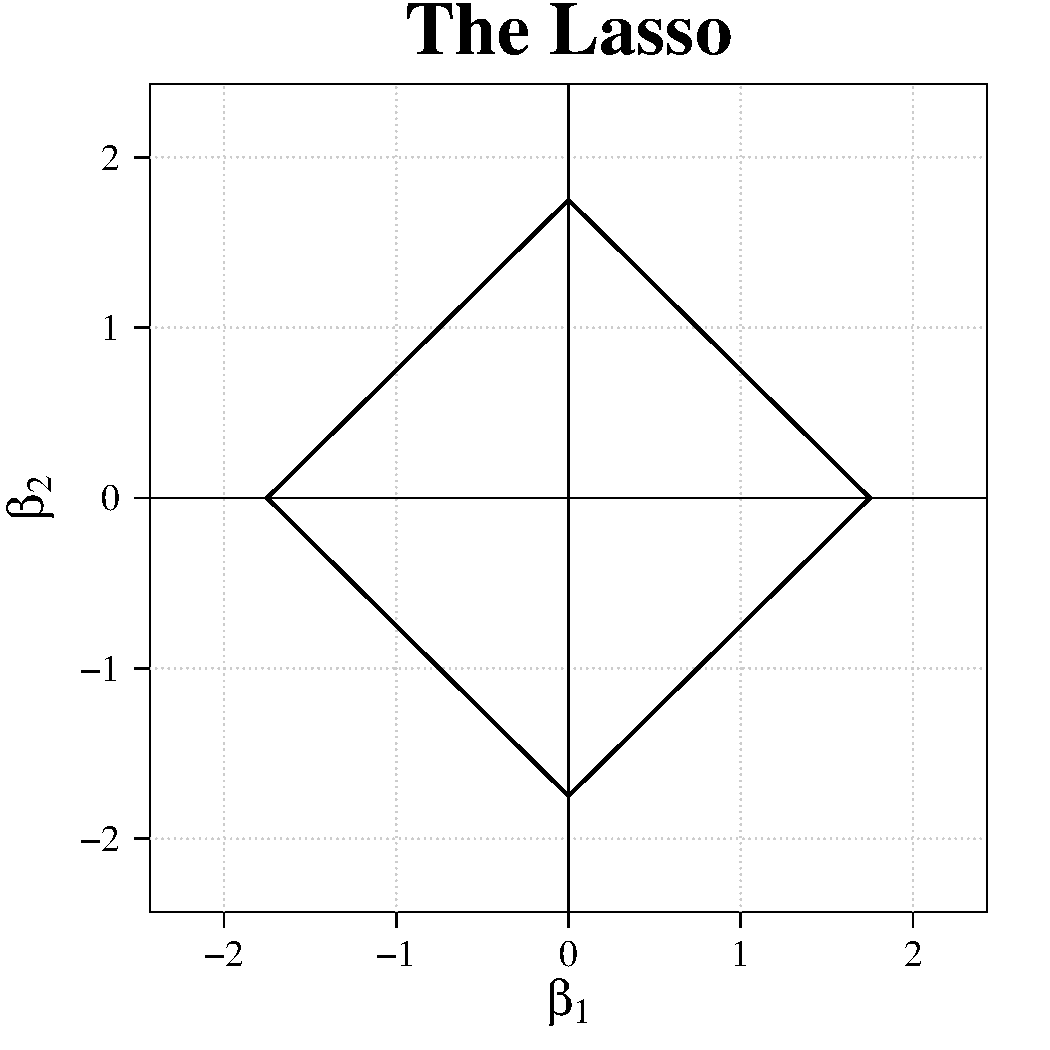
\includegraphics[width = 0.33\textwidth]{cont_lasso.pdf}
    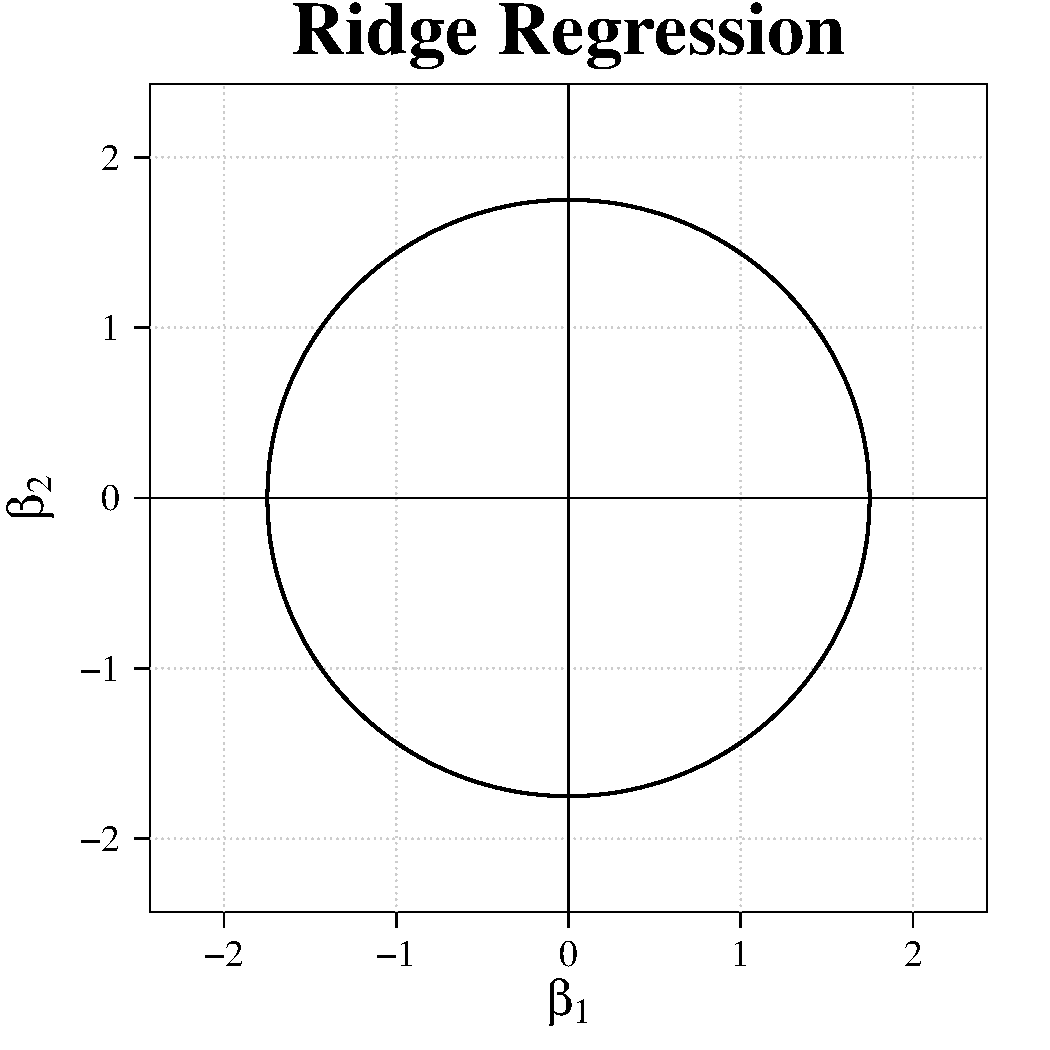
\includegraphics[width = 0.33\textwidth]{cont_ridge.pdf}
    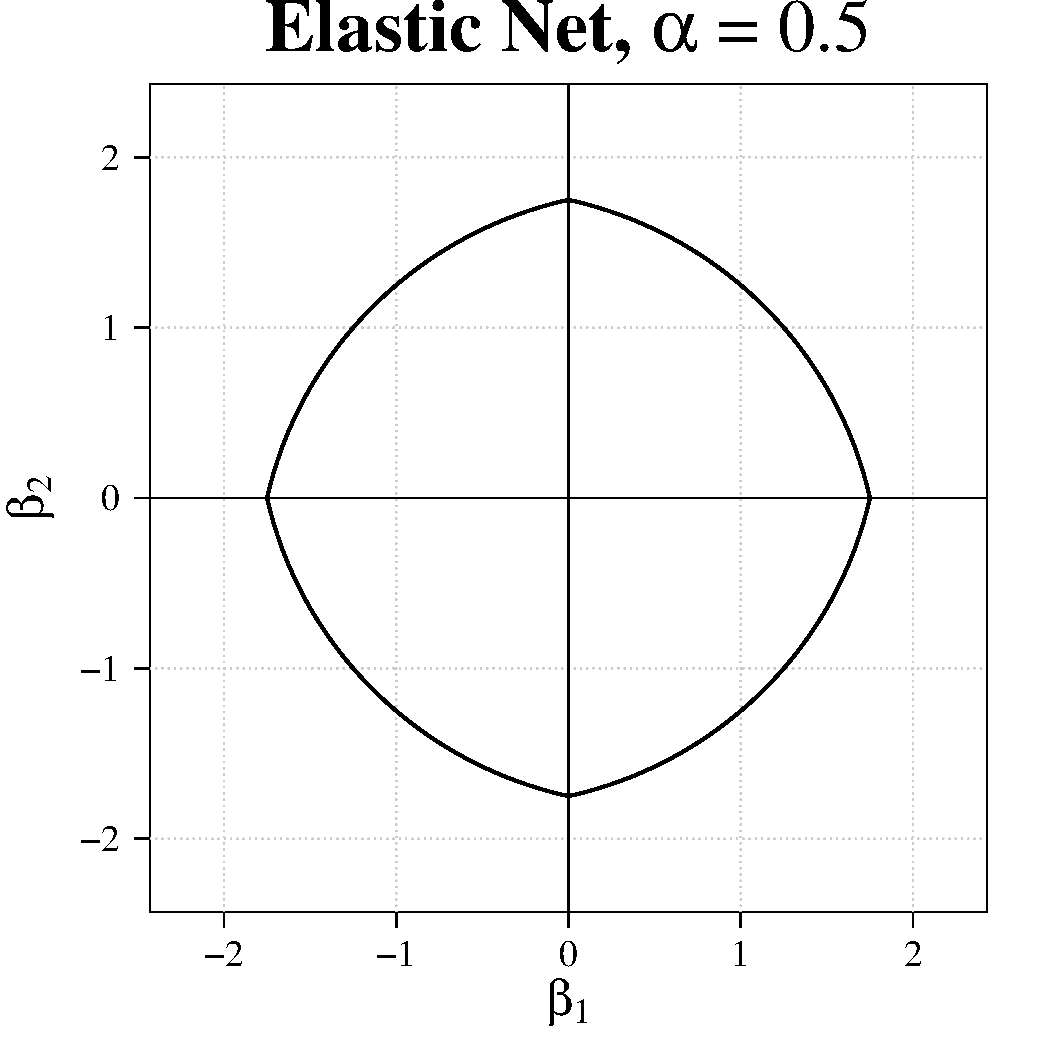
\includegraphics[width = 0.33\textwidth]{cont_enet.pdf}
    \caption{Contour plots for various regularization techniques for two predictors.}
    \label{mult_cont}
\end{figure} %\pause

In the special case of two predictors, i.e. $\bm{\beta} = (\beta_1,\beta_2)$, the estimated coefficients $\hat{\bm{\beta}}$ will lie on the \mydef{contour line} of the shrinkage penalty. %\pause

Gives some intuition about what type of shrinkage each method performs! %\pause 
\Laughey[1.25][yellow][pink]
    
\end{frame}

\begin{frame}{The Group Setting}

When you have a data matrix $\mathbf{X}$, it is possible that each of the predictors belong to different \mydef{groups}. %\pause

For example, let's say our data matrix $\mathbf{X}$ has $3$ observations and $6$ predictors, and is split up into four different groups. 
\begin{align*}
    \mathbf{X} &=
\begin{tikzpicture}[baseline=(m-2-1.base)]
        \matrix [matrix of math nodes,left delimiter=(,right delimiter=),
        ampersand replacement=\&] (m)
        {
            x_{1,1} \& x_{1,2} \& x_{1,3} \& x_{1,4} \& x_{1,5} \& x_{1,6} \\%[-1.5ex]               
            x_{2,1} \& x_{2,2} \& x_{2,3} \& x_{2,4} \& x_{2,5} \& x_{2,6} \\               
            x_{3,1} \& x_{3,2} \& x_{3,3} \& x_{3,4} \& x_{3,5} \& x_{3,6} \\           
        };  
        \begin{scope}[on background layer]
        \draw[color=Pink3, fill = Pink3, fill opacity = 0.25, rounded corners] (m-1-1.north west) -- (m-1-1.north east) -- (m-3-1.south east) -- (m-3-1.south west) -- cycle;
        \draw[color=SteelBlue3, fill = SteelBlue3, fill opacity = 0.25, rounded corners] (m-1-2.north west) -- (m-1-3.north east) -- (m-3-3.south east) -- (m-3-2.south west) -- cycle;
        \draw[color=orange, fill = orange, fill opacity = 0.25, rounded corners] (m-1-4.north west) -- (m-1-5.north east) -- (m-3-5.south east) -- (m-3-4.south west) -- cycle;
        \draw[color=Green4, fill = Green4, fill opacity = 0.25, rounded corners] (m-1-6.north west) -- (m-1-6.north east) -- (m-3-6.south east) -- (m-3-6.south west) -- cycle;
        \end{scope}
        \draw [decorate, decoration = {brace, amplitude = 5pt, mirror, raise = 2mm}, white] (m-3-1.south west) -- (m-3-1.south east) node[midway, yshift = -1em, align = center, black]{$\mathcal{G}_1$};
        \draw [decorate, decoration = {brace, amplitude = 5pt, mirror, raise = 2mm}, white] (m-3-2.south west) -- (m-3-3.south east) node[midway, yshift = -1em, align = center, black]{$\mathcal{G}_2$};
        \draw [decorate, decoration = {brace, amplitude = 5pt, mirror, raise = 2mm}, white] (m-3-4.south west) -- (m-3-5.south east) node[midway, yshift = -1em, align = center, black]{$\mathcal{G}_3$};
        \draw [decorate, decoration = {brace, amplitude = 5pt, mirror, raise = 2mm}, white] (m-3-6.south west) -- (m-3-6.south east) node[midway, yshift = -1em, align = center, black]{$\mathcal{G}_4$};
\end{tikzpicture}
\end{align*} %\pause

Note here that we have assumed that the groups do not \mydef{overlap}, so no predictor can be in two groups at once. %\pause

There are two ways to determine these groups: %\pause
\begin{enumerate}
    \item They are known to us from subject matter expertise. %\pause
    \item We can use various \mydef{clustering} techniques to determine them ourselves! %\pause
\end{enumerate}

We can use these groups to make predictions, as opposed to using the predictors individually!

\end{frame}

\begin{frame}{Clustering}

The goal of \mydef{clustering} is to split the data into \mydef{clusters}, or \mydef{subgroups}. %\pause
\begin{itemize}
    \item We want the observations \textit{within the same cluster} to be similar to each other, and observations \textit{within different clusters} to be different from each other. %\pause
    \item Clustering is a type of \mydef{unsupervised learning} method, where there is no response $\mathbf{y}$ that can be measured. %\pause
\end{itemize}

There are several different types of clustering algorithms. %\pause
\begin{itemize}
    \item e.g. K-means clustering, hierarchical clustering, spectral clustering. %\pause
    \item While the methodology for each is different, there is currently no consensus as to which method is the ``best.'' %\pause
\end{itemize}

We will be focusing on \mydef{K-means clustering}. %\pause
\begin{itemize}
    \item The observations $\bm{x}_i$ are split into $K$ \textit{non-overlapping} clusters $C_1, \ldots, C_K$. %\pause
    \item The clusters are chosen by minimizing the \mydef{within-cluster variation}, 
    \begin{align*}
        J(C_1, \ldots, C_K) = \sum_{k=1}^K \frac{1}{|C_k|} \sum_{i,i' \in C_k} \| \bm{x}_{i} - \bm{x}_{i'} \|_2^2.
    \end{align*} %\pause
    \item There are iterative algorithms that can easily solve this optimization problem!
\end{itemize}

%\begin{itemize}
%    \item A good clustering occurs when the \mydef{within-cluster variation} is as small as possible. Within-cluster variation is defined as 
%    \begin{align*}
%        \underset{C_1,\ldots,C_K}{\mathrm{argmin}} \left\{ \sum_{k=1}^K \frac{1}{|C_k|} \sum_{i,i' \in C_k} \sum_{j=1}^p (x_{ij}-x_{i',j})^2 \right\}
%    \end{align*}
%\end{itemize}

\end{frame}

\begin{frame}{More on K-Means Clustering}

\begin{figure}
    \centering
    \includegraphics[width = 0.33\textwidth]{clus_2.pdf}
    \includegraphics[width = 0.33\textwidth]{clus_3.pdf}
    \includegraphics[width = 0.33\textwidth]{clus_4.pdf}
    \caption{Clustering the same data with varying numbers of clusters.}
    \label{mult_cluster}
\end{figure} %\pause

How is the number of clusters chosen? There are several methods: %\pause
\begin{itemize}
    \item We can just arbitrarily choose them. %\pause
    \item Use subject matter expertise. %\pause
    \item Several criterion functions exist, such as the \mydef{GAP statistic} \cite{tibshirani2001estimating}.
\end{itemize}
    
\end{frame}


\begin{frame}{The Group Lasso}

Let's suppose that the $p$ predictors are divided into $L$ non-overlapping groups. Let $\mathbf{X}_{\ell}$ be the data matrix associated with group $\ell$, and let $p_{\ell}$ be the size of group $\ell$. %\pause

The \mydef{group lasso} (gLasso) \cite{yuan2006model} %seeks to minimize the members of a predetermined group of predictors together
imposes an $\ell_2$ norm on each of the group coefficient vectors! It minimizes the loss function 
\begin{align*}
    J(\bm{\beta}_1,\ldots,\bm{\beta}_L) = \frac{1}{2} \| \mathbf{y}  - \sum_{\ell=1}^L \mathbf{X}_{\ell} \bm{\beta}_{\ell} \|_2^2 + \lambda \sum_{\ell=1}^L \sqrt{p_{\ell}} \| \bm{\beta}_{\ell} \|_2.
\end{align*} %\pause
This is a generalization of the lasso, hence the name. %\pause

The gLasso acts like the lasso \textit{among groups} and acts like ridge regression \textit{within groups}. %\pause
\begin{itemize}
    \item In other words, any irrelevant \textit{clusters} will be forced to zero. %\pause
    \item However, \textit{within} those clusters, the estimated coefficients will all be nonzero. %\pause
    \item So its ``all or nothing,'' either all of the coefficients within a group are set to zero, or none of them are! %\pause
\end{itemize}

What if we want sparsity \textit{within} the clusters? 
    
\end{frame}

\begin{frame}{Contour Plots}

\begin{figure}[ht]

\centering
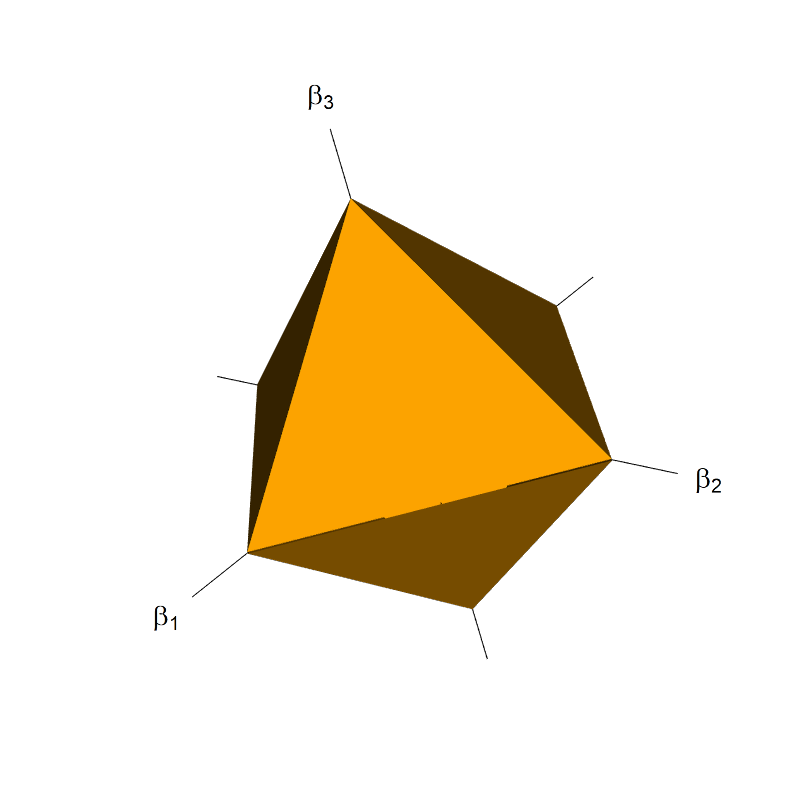
\includegraphics[width = 0.33\textwidth]{3D_lasso_contour.png}
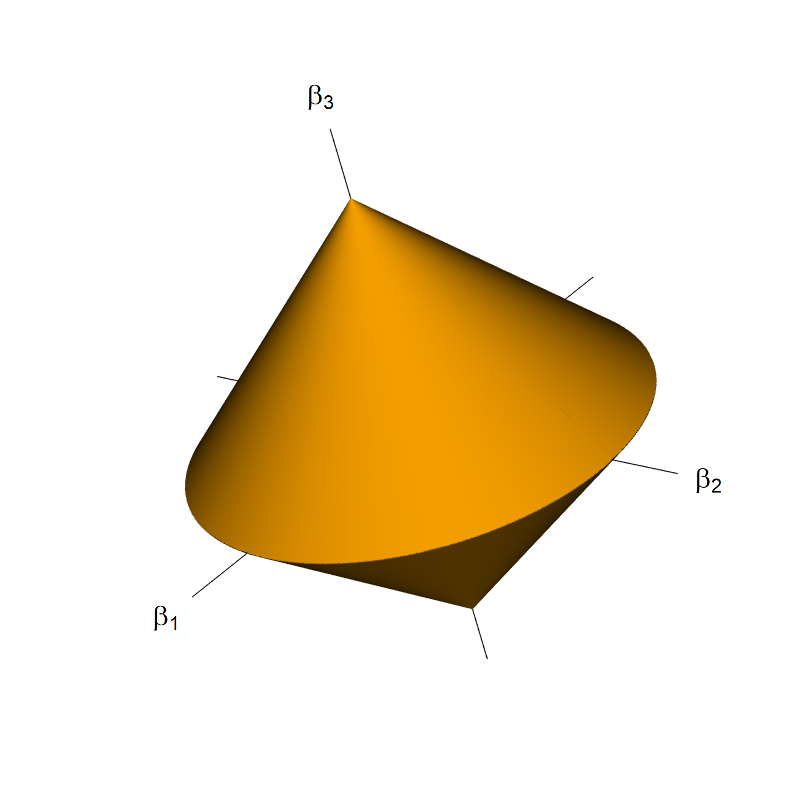
\includegraphics[width = 0.33\textwidth]{3D_glasso_contour.png}
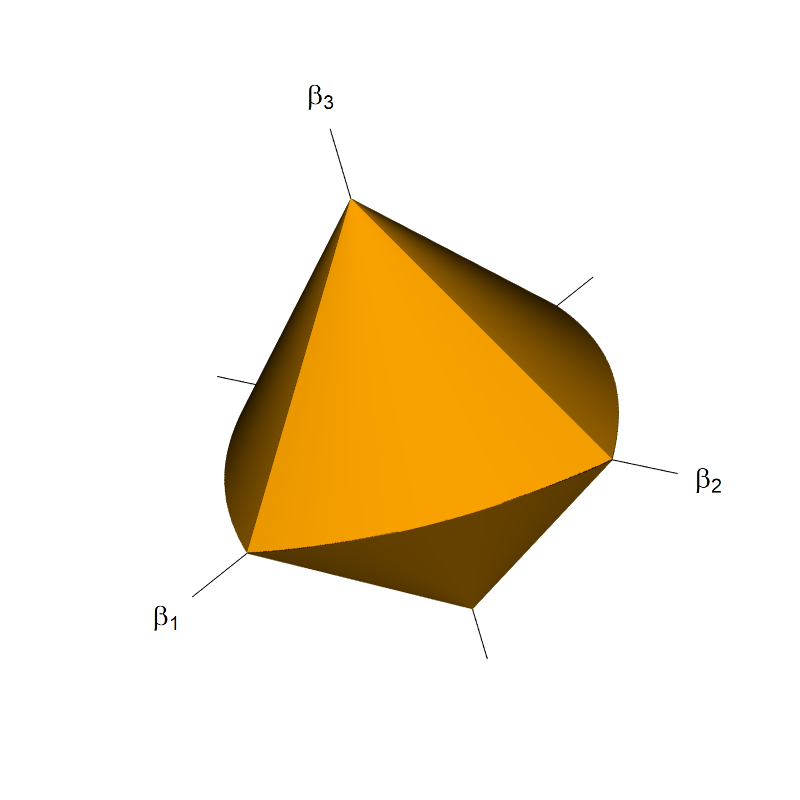
\includegraphics[width = 0.33\textwidth]{3D_sglasso_contour.png}

\caption{Contour lines for the lasso, the gLasso, and the sgLasso for three predictors.}

\end{figure}

In the special case of three predictors, i.e. $\bm{\beta}=(\beta_1,\beta_2,\beta_3)$, the estimated coefficients will lie on the \mydef{contour ball} of the shrinkage penalty. %\pause

In this example, there are two clusters, with $\bm{\beta}_1 = (\beta_1,\beta_2)$ and $\bm{\beta}_2 = \beta_3$. We can see how within the first cluster, the gLasso imposes an $\ell_2$ penalty, but among different groups it imposes an $\ell_1$ penalty.

For the sgLasso, $\alpha = 0.5$.
    
\end{frame}

\begin{frame}{The Supervised Group Lasso}

The \mydef{supervised group lasso} (sgLasso) \cite{ma2007supervised} is a two-step process that involves both the lasso and the group lasso. %\pause
\begin{enumerate}
    \item First, the group lasso is fit to determine which clusters in the data are significant. %\pause
    \item Next, the lasso is fit for each of the clusters individually. %\pause
\end{enumerate}
The resulting model selects both the most important clusters \textit{and} the most important predictors from each cluster, so the model is very interpretable! %\pause

For example, from the previous clusters, let's say that after sgLasso is used, the first group is shrunken to zero, and the second predictor in the second group is set to zero. 
\begin{align*}
\begin{tikzpicture}[baseline=(m-2-1.base)]
        \matrix [matrix of math nodes,
        ampersand replacement=\&] (m)
        {
            x_{1,1} \& x_{1,2} \& x_{1,3} \& x_{1,4} \& x_{1,5} \& x_{1,6} \\%[-1.5ex]               
            x_{2,1} \& x_{2,2} \& x_{2,3} \& x_{2,4} \& x_{2,5} \& x_{2,6} \\               
            x_{3,1} \& x_{3,2} \& x_{3,3} \& x_{3,4} \& x_{3,5} \& x_{3,6} \\           
        };  
        \begin{scope}[on background layer]
        \draw[color=Pink3, fill = Pink3, fill opacity = 0.25, rounded corners] (m-1-1.north west) -- (m-1-1.north east) -- (m-3-1.south east) -- (m-3-1.south west) -- cycle;
        \draw[color=SteelBlue3, fill = SteelBlue3, fill opacity = 0.25, rounded corners] (m-1-2.north west) -- (m-1-3.north east) -- (m-3-3.south east) -- (m-3-2.south west) -- cycle;
        \draw[color=orange, fill = orange, fill opacity = 0.25, rounded corners] (m-1-4.north west) -- (m-1-5.north east) -- (m-3-5.south east) -- (m-3-4.south west) -- cycle;
        \draw[color=Green4, fill = Green4, fill opacity = 0.25, rounded corners] (m-1-6.north west) -- (m-1-6.north east) -- (m-3-6.south east) -- (m-3-6.south west) -- cycle;
        \end{scope}
        \draw [decorate, decoration = {brace, amplitude = 5pt, mirror, raise = 2mm}, white] (m-3-1.south west) -- (m-3-1.south east) node[midway, yshift = -1em, align = center, black]{$\mathcal{G}_1$};
        \draw [decorate, decoration = {brace, amplitude = 5pt, mirror, raise = 2mm}, white] (m-3-2.south west) -- (m-3-3.south east) node[midway, yshift = -1em, align = center, black]{$\mathcal{G}_2$};
        \draw [decorate, decoration = {brace, amplitude = 5pt, mirror, raise = 2mm}, white] (m-3-4.south west) -- (m-3-5.south east) node[midway, yshift = -1em, align = center, black]{$\mathcal{G}_3$};
        \draw [decorate, decoration = {brace, amplitude = 5pt, mirror, raise = 2mm}, white] (m-3-6.south west) -- (m-3-6.south east) node[midway, yshift = -1em, align = center, black]{$\mathcal{G}_4$};
\end{tikzpicture}
\implies
\begin{tikzpicture}[baseline=(m-2-1.base)]
        \matrix [matrix of math nodes,
        ampersand replacement=\&] (m)
        {
            x_{1,2} \& x_{1,4} \& x_{1,5} \& x_{1,6} \\ 
            x_{2,2} \& x_{2,4} \& x_{2,5} \& x_{2,6} \\ 
            x_{3,2} \& x_{3,4} \& x_{3,5} \& x_{3,6} \\           
        };  
        \begin{scope}[on background layer]
        \draw[color=SteelBlue3, fill = SteelBlue3, fill opacity = 0.25, rounded corners] (m-1-1.north west) -- (m-1-1.north east) -- (m-3-1.south east) -- (m-3-1.south west) -- cycle;
        \draw[color=orange, fill = orange, fill opacity = 0.25, rounded corners] (m-1-2.north west) -- (m-1-3.north east) -- (m-3-3.south east) -- (m-3-2.south west) -- cycle;
        \draw[color=Green4, fill = Green4, fill opacity = 0.25, rounded corners] (m-1-4.north west) -- (m-1-4.north east) -- (m-3-4.south east) -- (m-3-4.south west) -- cycle;
        \end{scope}
        \draw [decorate, decoration = {brace, amplitude = 5pt, mirror, raise = 2mm}, white] (m-3-1.south west) -- (m-3-1.south east) node[midway, yshift = -1em, align = center, black]{$\mathcal{G}_2$};
        \draw [decorate, decoration = {brace, amplitude = 5pt, mirror, raise = 2mm}, white] (m-3-2.south west) -- (m-3-3.south east) node[midway, yshift = -1em, align = center, black]{$\mathcal{G}_3$};
        \draw [decorate, decoration = {brace, amplitude = 5pt, mirror, raise = 2mm}, white] (m-3-4.south west) -- (m-3-4.south east) node[midway, yshift = -1em, align = center, black]{$\mathcal{G}_4$};
\end{tikzpicture}
\end{align*}

\end{frame}

\begin{frame}{The Sparse Group Lasso}

The \mydef{sparse group lasso} (spgLasso) %\parentcite{friedman2010note} 
\cite{friedman2010note} 
attempts to combine the lasso and the gLasso simultaneously. It minimizes the loss function 
\begin{align*}
    J(\bm{\beta}) = \frac{1}{2} \| \mathbf{y}  - \sum_{\ell=1}^L \mathbf{X}_{\ell} \bm{\beta}_{\ell} \|_2^2 + \lambda \| \bm{\beta} \|_1 + \theta \sum_{\ell=1}^L \sqrt{p_{\ell}} \| \bm{\beta}_{\ell} \|_2.
\end{align*} 
Here, $\lambda$ and $\theta$ are two separate tuning parameters. %\pause
Can also be written as 
\begin{align*}
    J(\bm{\beta}) = \frac{1}{2} \| \mathbf{y}  - \sum_{\ell=1}^L \mathbf{X}_{\ell} \bm{\beta}_{\ell} \|_2^2 + \lambda \Big[ \alpha \| \bm{\beta} \|_1 + (1 - \alpha) \sum_{\ell=1}^L \sqrt{p_{\ell}} \| \bm{\beta}_{\ell} \|_2 \Big].
\end{align*},
where $\alpha = \frac{\theta}{\lambda + \theta}$

As opposed to the two-step process of the sgLasso, the spgLasso promotes sparsity among the clusters and within the clusters in one step!
    
\end{frame}

\begin{frame}{Principal Component Analysis}

\mydef{Principal component analysis} is a technique for using the principal components of a data set to explain the variance of the data. %\pause
\begin{itemize}
    \item They are a \mydef{linear combination} of the predictors in the data set $\mathbf{X}$. %\pause
\end{itemize}

We will be exploiting their variance-explaining property by using the principal components to help us make predictions. %\pause

The (economy) \mydef{singular value decomposition} (SVD) of a data matrix $\mathbf{X}$ with $m = \mathrm{rank}(\mathbf{X})$ is given by 
\begin{align*}
    \mathbf{X} = \mathbf{U} \mathbf{S} \mathbf{V}^T,
\end{align*} 
where $\mathbf{U}_{n \times m}$ and $\mathbf{V}_{m \times p}$ are orthogonal matrices and $\mathbf{S}_{m \times m}$ is a diagonal matrix. %\pause
\begin{itemize}
    \item The columns of $\mathbf{V}$ are the \mydef{right singular vectors} and the columns of $\mathbf{U}$ are the \mydef{left singular vectors}. %\pause
    \item The \mydef{singular values} of $\mathbf{X}$ are stored in the diagonal of $\mathbf{S}$ in descending order, such that $s_1 \ge \ldots \ge s_m > 0$. %\pause
    \item The columns of $\mathbf{V}$ are the \mydef{principal axes} of $\mathbf{X}$. %\pause
    \item The columns of $\mathbf{US}$ are the \mydef{principal components}.
\end{itemize}
    
\end{frame}

\begin{frame}{The Principal Components Lasso}

Let $m_{\ell} = \mathrm{rank}(\mathbf{X}_{\ell})$ and $(\mathbf{V}_{\ell}, s_{\ell})$ be the right singular values and singular vectors of $\mathbf{X}_{\ell}$. %\pause

The \mydef{principal components lasso} (pcLasso) \cite{2018arXiv181004651T} is a state-of-the-art method that strongly biases the shrinkage toward the leading principal components. It minimizes the loss function
\begin{align*}
    J(\bm{\beta}) = \frac{1}{2} \| \mathbf{y}  - \mathbf{X} \bm{\beta} \|_2^2 + \lambda \| \bm{\beta} \|_1 + \frac{\theta}{2} \sum_{\ell=1}^L \sqrt{p_{\ell}} \bm{\beta}_{\ell}^T \Big(\mathbf{V}_{\ell} \mathbf{S}_{s_{\ell 1}^2 - s_{\ell j}^2} \mathbf{V}_{\ell}^T \Big) \bm{\beta}_{\ell}.
\end{align*} %\pause
Here, $\displaystyle \mathbf{S}_{s_{\ell 1}^2 - s_{\ell j}^2}$ is an $m_{\ell} \times m_{\ell}$ diagonal matrix whose entries correspond to $s_{\ell 1}^2 - s_{\ell j}^2$ for $j=1,\ldots,m_{\ell}$, and is known as the \mydef{pcLasso penalty}. %\pause
\begin{itemize}
    \item This has the effect of imposing a smaller penalty in the direction of the leading singular vector, and a larger penalty in the direction of the other singular vectors. %\pause
    \item The smaller the non-leading singular vectors are, the larger the penalty! %\pause
    \item $\theta \to \infty$ causes the pcLasso penalty to carry more weight, biasing the estimates in the direction of the leading principal component. %\pause
    \item $\lambda \to \infty$ causes the lasso penalty to carry more weight, causing the pcLasso to act similar to the lasso.
\end{itemize}
    
\end{frame}

\begin{frame}{Contour Plots}

\begin{figure}
    \centering
    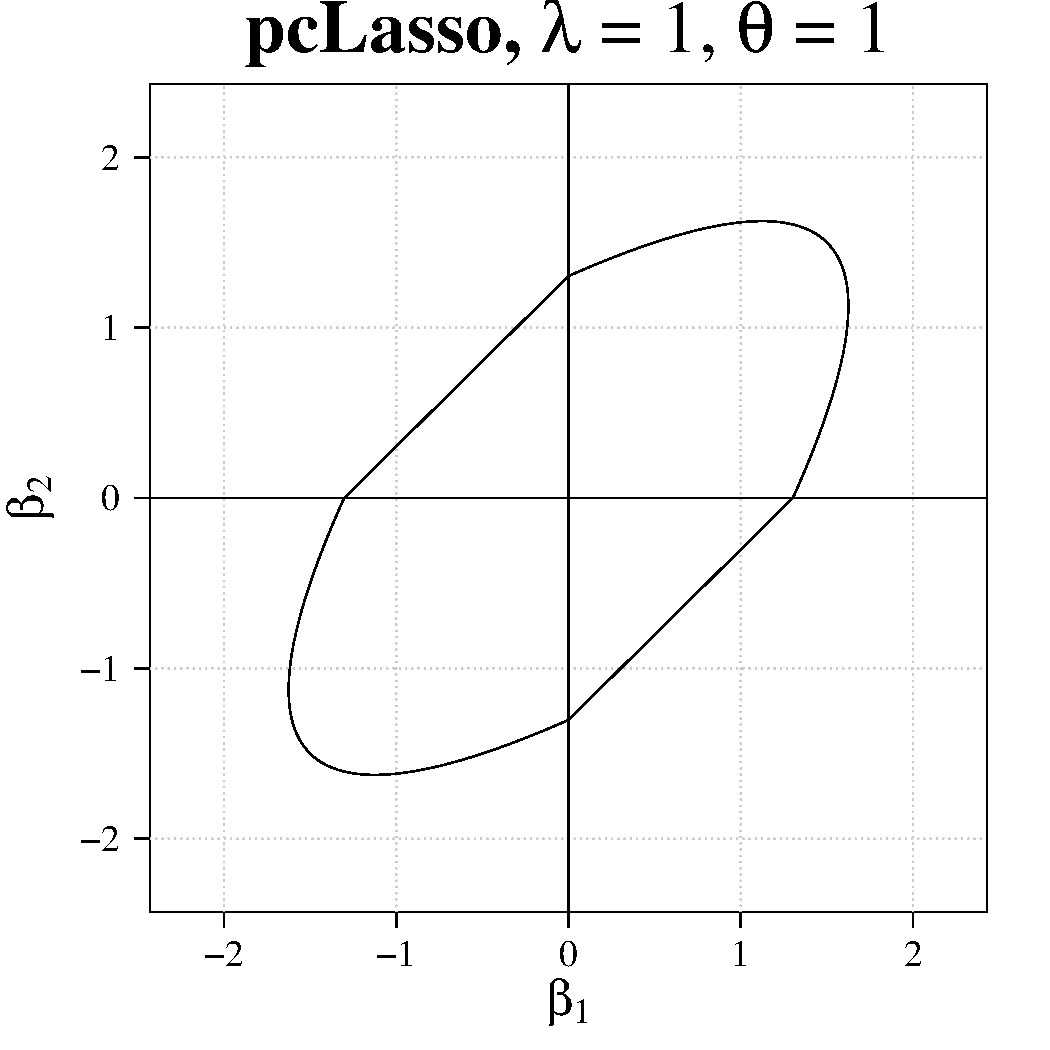
\includegraphics[width = 0.33\textwidth]{Presentation/cont_pcLasso_t3.pdf}
    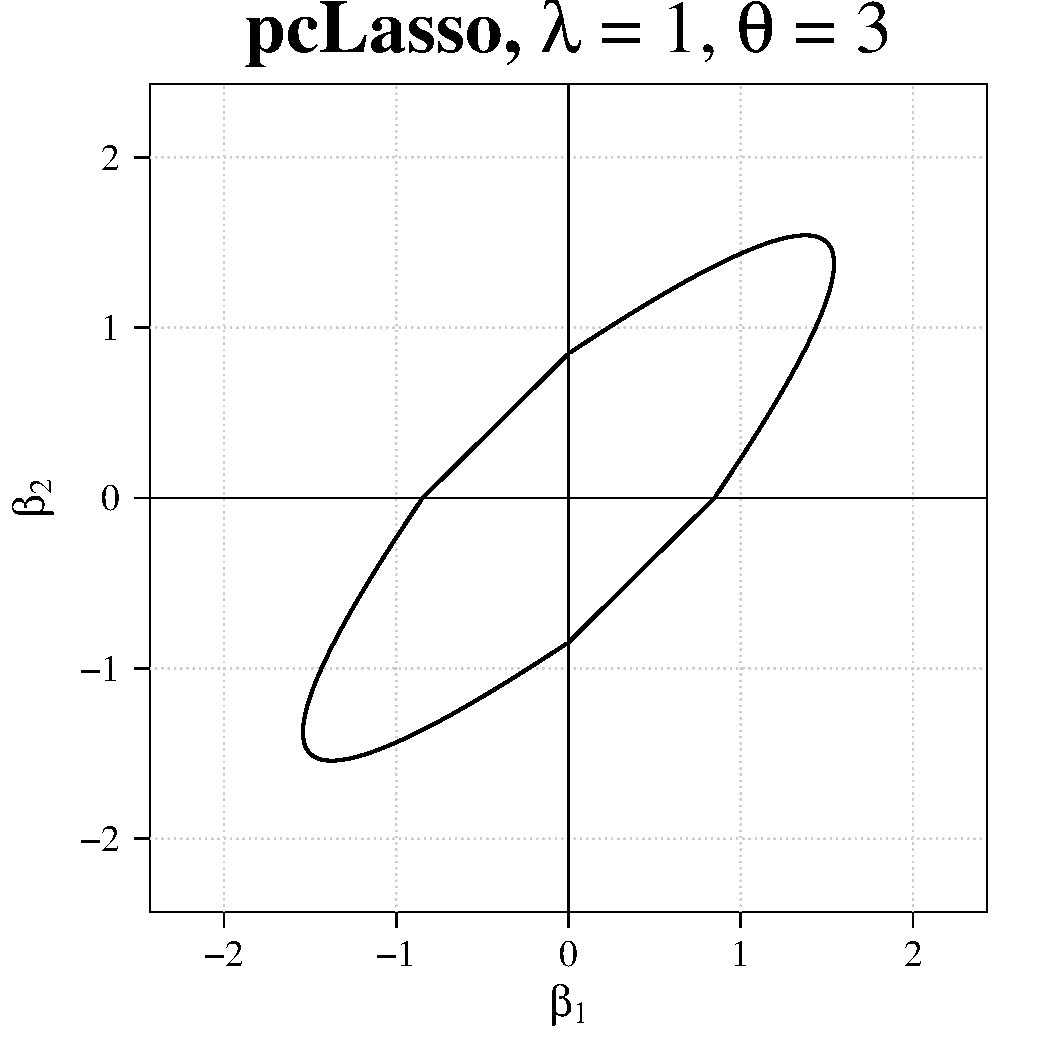
\includegraphics[width = 0.33\textwidth]{Presentation/cont_pcLasso_t2.pdf}
    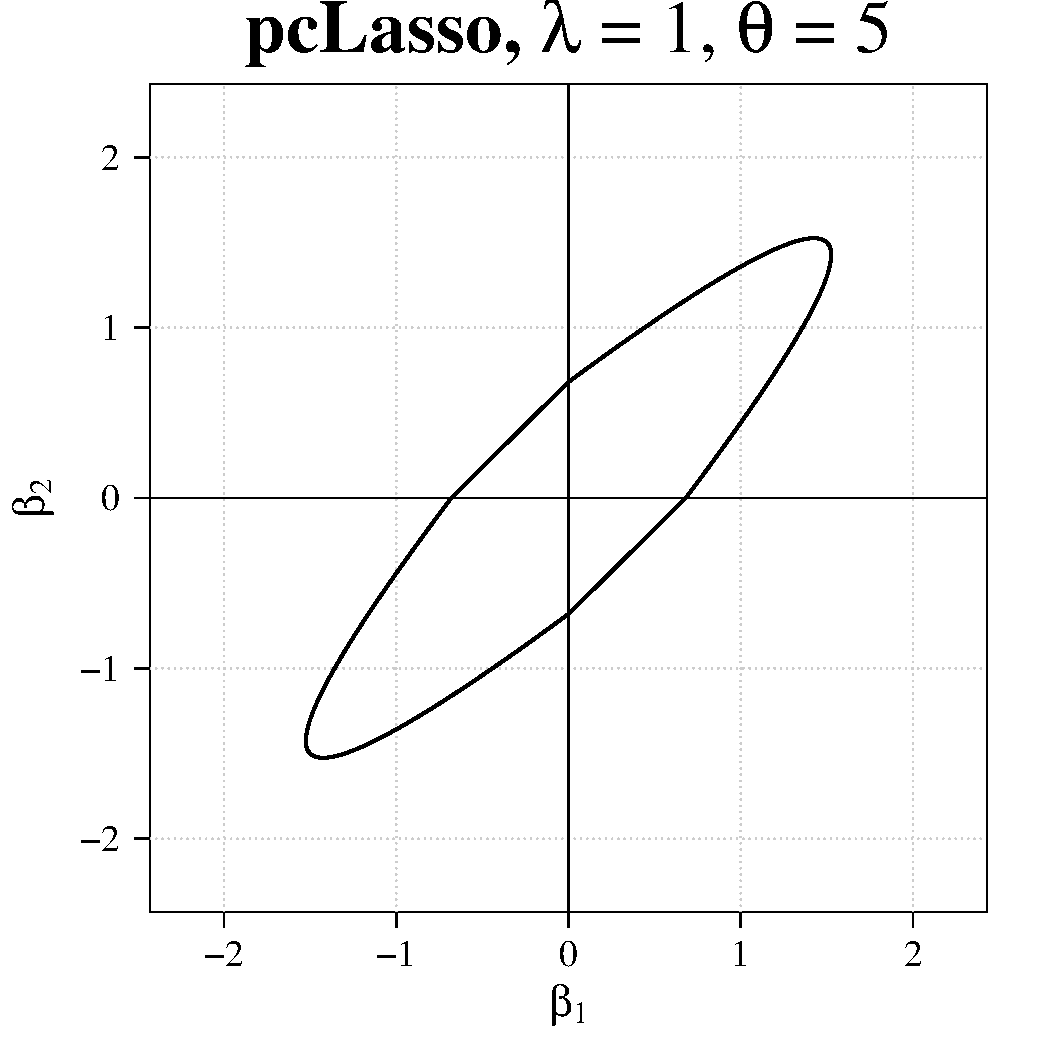
\includegraphics[width = 0.33\textwidth]{Presentation/cont_pcLasso_t1.pdf}
    
    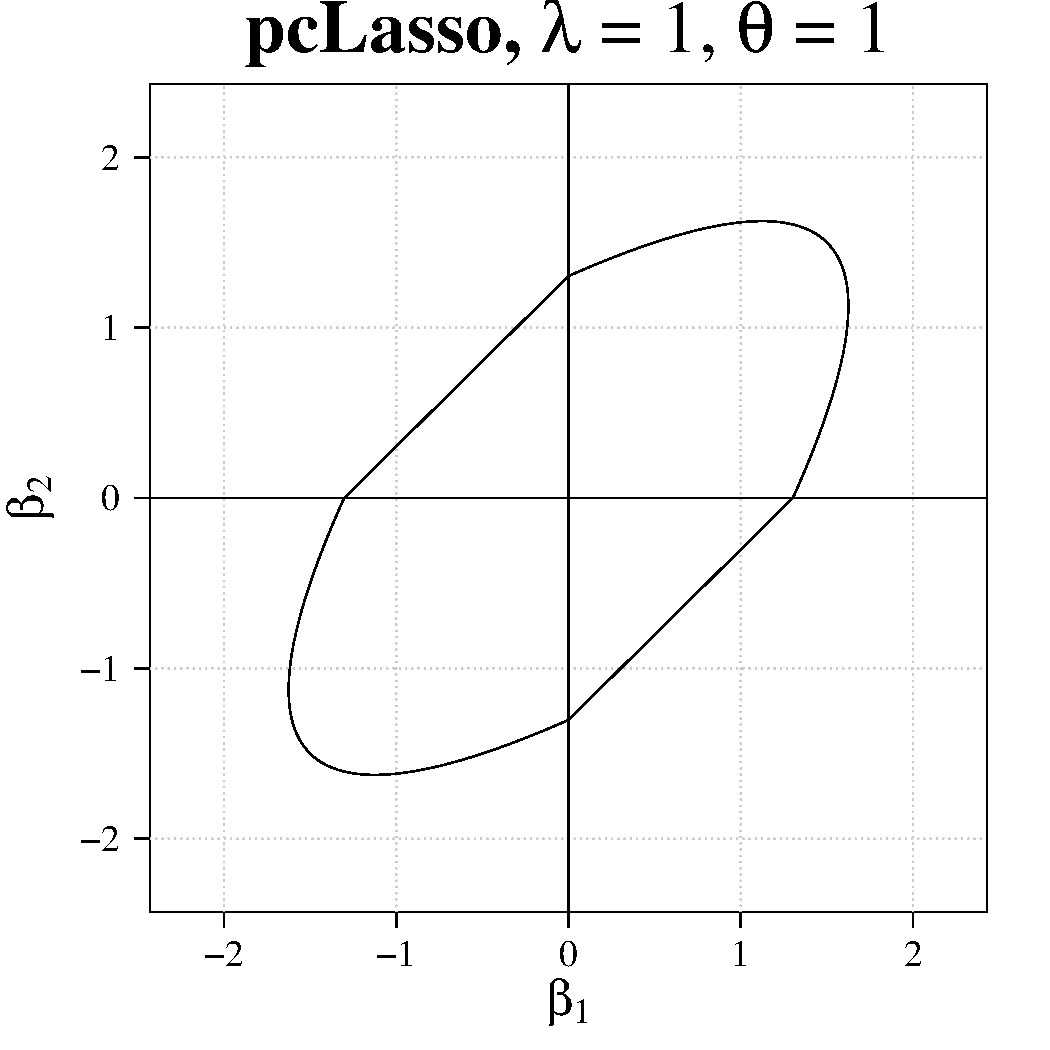
\includegraphics[width = 0.33\textwidth]{Presentation/cont_pcLasso_l3.pdf}
    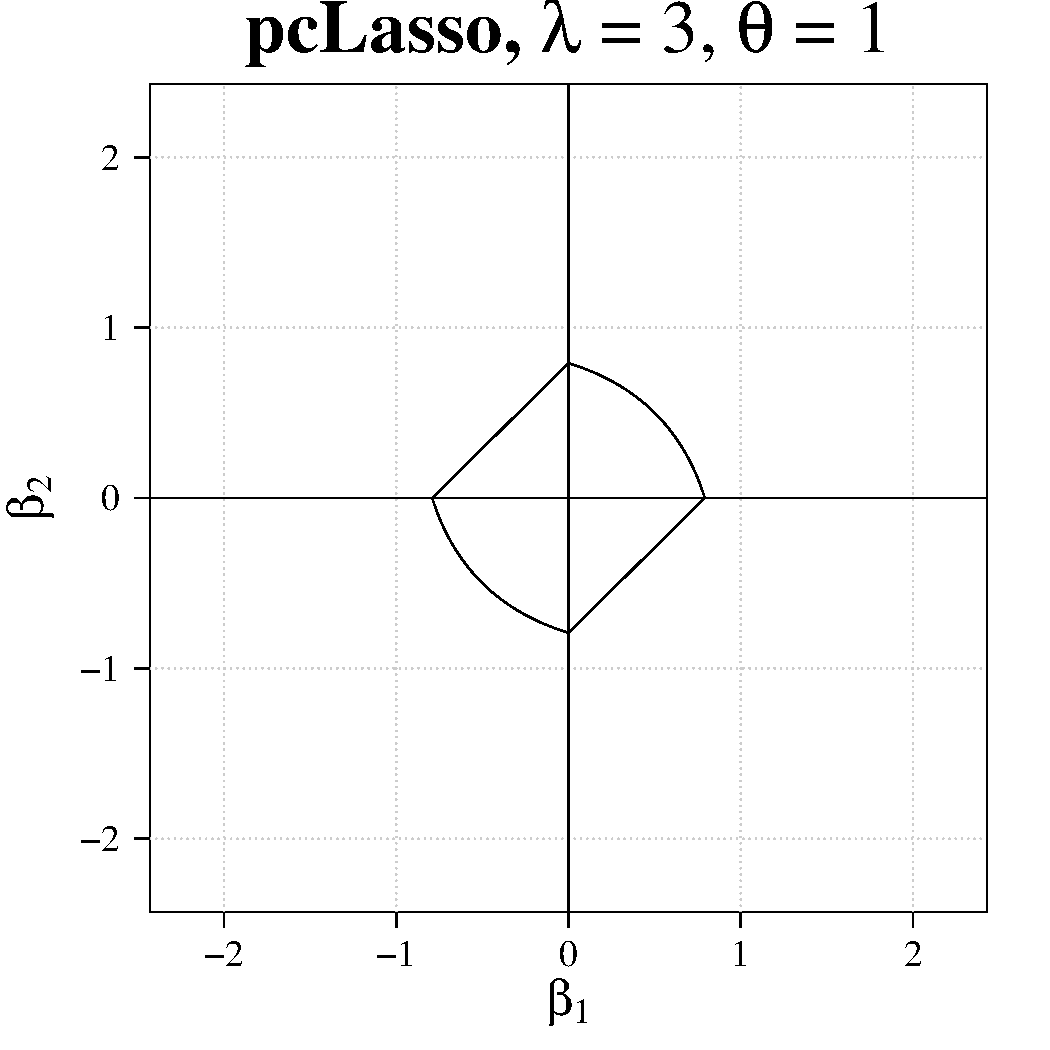
\includegraphics[width = 0.33\textwidth]{Presentation/cont_pcLasso_l2.pdf}
    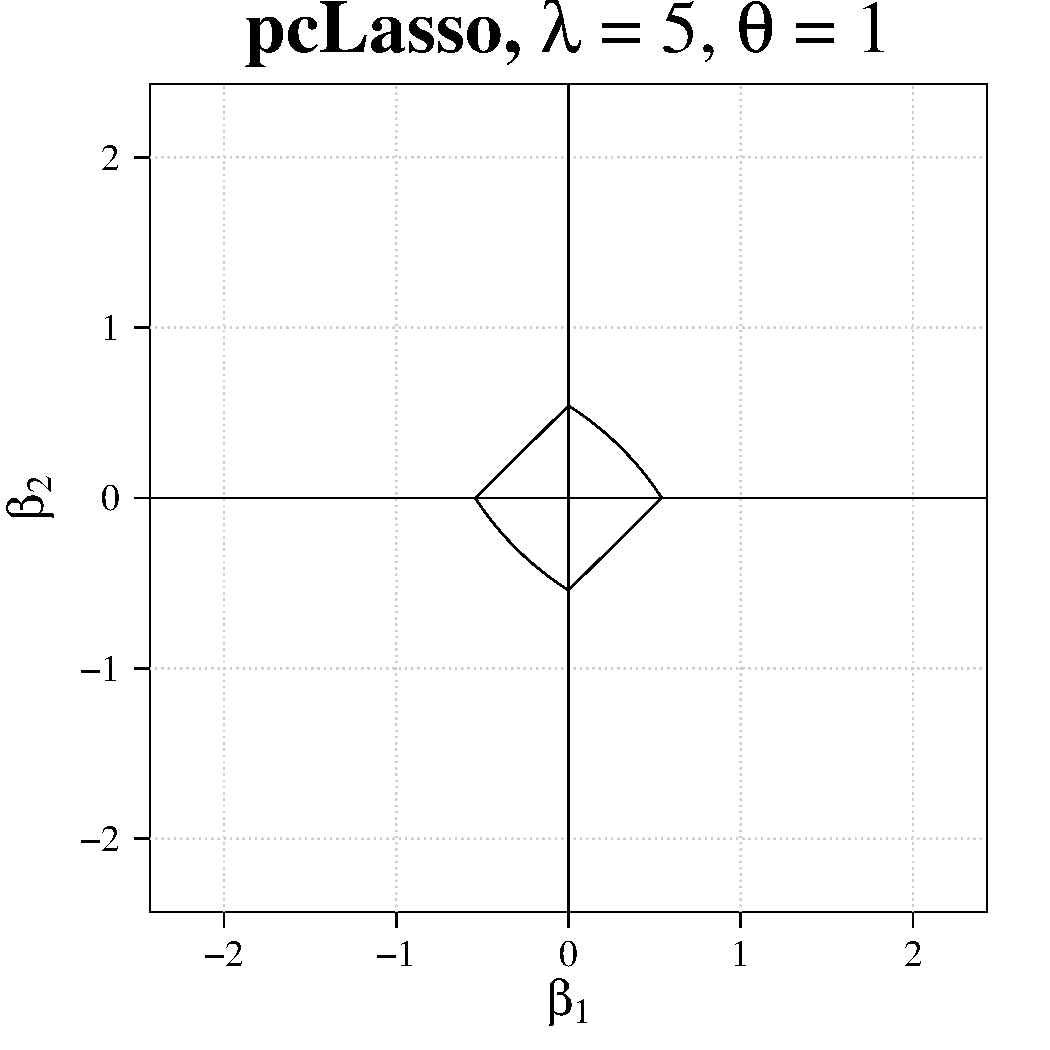
\includegraphics[width = 0.33\textwidth]{Presentation/cont_pcLasso_l1.pdf}
    \caption{Contour plots for pcLasso for various tuning parameters for two predictors.}
    \label{pcLasso_cont}
\end{figure} %\pause
    
\end{frame}

\begin{frame}{What We're Doing Now}

A paper we are working to reproduce, \cite{ma2007supervised}, is using regularization with genomic data. %\pause
\begin{itemize}
    \item The {\color{SteelBlue4} \texttt{colon}} data set observes the outputs of 2000 different genes for 62 different tissue samples. So $n=62$ and $p=2000$. %\pause
    \item The response is binary: the tissue sites either have cancer or do not. %\pause
    \item The goal is to predict the presence of cancer given the expression of the genes, as well as which genes are most important! %\pause
\end{itemize}

So what is so special about this genomic data? %\pause
\begin{itemize}
    \item Genes have a natural structure that can be exploited! %\pause
    \item So we are interested in important clusters, as well as important genes within each cluster. %\pause
\end{itemize}

The paper used the lasso, the gLasso, the sgLasso, and $K$-means clustering. %\pause

The paper is older (2007), so newer techniques (e.g. pcLasso, 2018) may result in higher prediction accuracy! 
    
\end{frame}

\begin{frame}{Ultimate Goal and Conclusions}

As it stands, we are currently looking for a data set to do our analysis on! %\pause
\Sadey[1.25][yellow] %\pause

``The best thing about being a statistician is that you get to play in everyone's backyard.''
\hfill $\sim$ John Tukey \hspace{0.4cm} %\pause

In other words, the applications of these statistical learning methods are endless! %\pause
\begin{itemize}
    \item e.g. Genomics, oceanography, environmental science, robotics, marketing, economics. %\pause
\end{itemize}

We are looking to find a data set and build a predictive model that is both accurate and interpretable. %\pause

During the process, we will be comparing various methods to see: %\pause
\begin{itemize}
    \item Which method results in a model that \textit{performs} the best. %\pause
    \item How the \textit{interpretability} of our model changes for each method. %\pause
\end{itemize}
    
\end{frame}


\begin{frame}[allowframebreaks]{References}

\bibliographystyle{apalike}
\bibliography{pres_sources}
    
\end{frame}









\end{document}



%%%%%%%%%%%%%%%%%%%%%%%%%%%%%%%%%%%%%%%%%%%%%%%%%%%%%%%%%%%%%%%
% HERE ARE THE CONTOUR PLOTS IN LATEX
%%%%%%%%%%%%%%%%%%%%%%%%%%%%%%%%%%%%%%%%%%%%%%%%%%%%%%%%%%%%%%%

\begin{figure}[ht]

\centering

\begin{tikzpicture}[scale=0.9]
\begin{axis}[
view = {112}{18},
grid=minor,
xlabel = $\beta_1$,
ylabel = $\beta_2$,
zlabel = $\beta_3$,
ticks = none,
axis lines=middle,
every axis x label/.style={
    at={(ticklabel* cs:1.2)},
    anchor=west,
},
every axis y label/.style={
    at={(ticklabel* cs:1.025)},
    anchor=west,
},
every axis z label/.style={
    at={(ticklabel* cs:1.14)},
    anchor=north,
},
inner axis line style={-},
xmin = -1.5, xmax = 1.5,
ymin = -1.35, ymax = 1.35,
zmin = -1.35, zmax = 1.35,
font=\normalsize,
xtick distance = 1,
ytick distance = 1,
ztick distance = 1,
]

\filldraw[Orange2] (0,0,1) -- (0,0.85,0) -- (1,0,0) -- cycle;
\filldraw[Orange4] (0,0,1) -- (0,-0.85,0) -- (1,0,0) -- cycle;
\filldraw[Orange4] (0,0,-1) -- (0,0.85,0) -- (1,0,0) -- cycle;
\filldraw[Auburn] (0,0,-1) -- (0,-0.85,0) -- (1,0,0) -- cycle;
\draw[black] (1,0,0) -- (1.49,0,0);

\end{axis}
\end{tikzpicture}
\hspace{0.5cm}
\begin{tikzpicture}[scale=0.9]
\begin{axis}[
%unit vector ratio=1 1 1,
view = {112}{18},
grid=minor,
xlabel = $\beta_1$,
ylabel = $\beta_2$,
zlabel = $\beta_3$,
ticks = none,
axis lines=middle,
every axis x label/.style={
    at={(ticklabel* cs:1.2)},
    anchor=west,
},
every axis y label/.style={
    at={(ticklabel* cs:1.05)},
    anchor=west,
},
every axis z label/.style={
    at={(ticklabel* cs:1.14)},
    anchor=north,
},
inner axis line style={-},
xmin = -1.5, xmax = 1.5,
ymin = -1.35, ymax = 1.35,
zmin = -1.35, zmax = 1.35,
font=\normalsize
]

% botton
\addplot3[domain=0:360,domain y=0:1,surf,shader=interp,
point meta={-2},
colormap={idnonthaveyourorange}{color=(Orange3!30!black) color=(Orange3)}] 
({y*cos(x)},{0.85*y*sin(x)},-1+y);
%({x*cos(deg(y))},{0.85*x*sin(deg(y))},{abs(x)-1});

% top
\addplot3[domain=0:360,domain y=0:1,surf,shader=interp,
point meta={atan2(x+y,1)*z},
colormap={idnonthaveyourorange}{%color=(black!10)
color=(Orange2!45!black) color=(Orange2)}] ({y*cos(x)},{0.85*y*sin(x)},1-y);

\draw (1,0,0) -- (1.5,0,0);
\draw (0,1,0) -- (0,1.5,0);

\draw[black] (1,0,0) -- (1.49,0,0);

\end{axis}
\end{tikzpicture}

\caption{Contour lines for the lasso and the gLasso for three predictors.}

\end{figure}